% vim: spell
\documentclass[10pt]{sigplanconf}

% The following \documentclass options may be useful:
%
% 10pt  To set in 10-point type instead of 9-point.
% 11pt  To set in 11-point type instead of 9-point.
% authoryear To obtain author/year citation style instead of numeric.

\usepackage{amsmath}
\usepackage{bbding}
\usepackage{pifont}
\usepackage{url}
\usepackage[pdftex]{graphicx}

\begin{document}

\conferenceinfo{PLATEAU '12}{October 21, Tucson (AZ)} 
\copyrightyear{2012} 
\copyrightdata{[to be supplied]}

%\titlebanner{banner above paper title} % These are ignored unless
%\preprintfooter{short description of paper} % 'preprint' option specified.

\title{Comparative Language Fuzz Testing}
\subtitle{Programming Languages vs. Fat Fingers}

\authorinfo{Diomidis Spinellis\and Vassilios Karakoidas}
  {Athens University of Economics and Business}
  {\{dds, bkarak\}@aueb.gr}

\maketitle

\begin{abstract}
We explore how programs written in ten popular programming languages
are affected by small changes of their source code.
This allows us to analyze the extend to which these languages
allow the detection of simple errors at compile or at run time.
Our study is based on a large corpus of programs written in several programming
languages systematically perturbed using a mutation-based fuzz generator.
The results we obtained
prove that languages with weak type systems are significantly
likelier than languages that enforce strong typing to let fuzzed programs
compile and run, and, in the end, produce erroneous results.
More importantly, our study also shows that comparative language fuzz testing
is a legitimate technique for evaluating programming language designs.
\end{abstract}

 \category{D.3.0}{Programming Languages}{General}

\terms
Reliability, Experimentation, Measurement

\keywords
Programming Languages; Fuzzing; Comparison; Rosetta Stone

\section{Introduction} % {{{1
A substitution of a comma with a period in project Mercury's working
{\sc fortran} code compromised the accuracy of the results,
rendering them unsuitable for longer orbital missions \cite{Brad89,Neu95}.
How probable are such events and how does a programming language's
design affect their likelihood and severity?

To study these questions we chose ten popular programming languages,
and a corpus of programs written in all of them.
We then constructed a source code mutation {\em fuzzer}:
a tool that systematically introduces diverse random perturbations
into the program's source code,
and examined whether the resultant source code had errors that
were detected at compile or runtime, and whether it produced
erroneous results.

In practice,
the errors that we artificially introduced into the source code can
crop up in a number of ways.
Mistyping---the ``fat fingers'' syndrome-- is one plausible source.
Other scenarios include
absent-mindedness,
automated refactorings gone awry
(especially in languages where such tasks cannot be reliably implemented),
unintended consequences from complex editor commands or
search-and-replace operations,
and even the odd cat walking over the keyboard.

The contribution of our work is twofold.
First, we describe a method for systematically evaluating the tolerance
of source code written in diverse programming languages to a particular
class of errors.
In addition, we apply this method to numerous tasks written in ten popular
programming languages,
and by analyzing tens of thousands of cases we present an overview of
the likelihood and impact of these errors among diverse languages.

In the remainder of this paper we
outline our methods (Section~\ref{sec:method}),
present and discuss our findings (Section~\ref{sec:results}),
compare our approach against related work (Section~\ref{sec:related}),
and conclude with proposals for further study (Section~\ref{sec:conclusions}).

\section{Methodology} % {{{1
\label{sec:method}

\begin{table}
\begin{center}
\begin{tabular}{ l l}
Language & Implementation \\
\hline
C 			& gcc 4.4.5 \\
C++ 		& g++ 4.4.5 \\
C\# 		& mono 2.6.7, CLI v2.0 \\
Haskell 	& ghc 6.12.1 \\
Java 		& OpenJDK 1.6.0\_18 \\
JavaScript 	& spidermonkey 1.8.0 \\
{\sc php} 		& {\sc php} 5.3.3-7 \\
Perl 		& perl 5.10.1 \\
Python 		& python 2.6.6 \\
Ruby 		& ruby 1.5.8 \\
\end{tabular}
\end{center}
\caption{Tested languages.}
\label{tab:langs}
\end{table}

We selected the languages to test based on a number of sources
collated in an {\sc ieee} Spectrum article \cite{Kin11}:
an index created by
{\sc tiobe}\footnote{\url{http://www.tiobe.com/index.php/content/paperinfo/tpci/index.html}} (a software research firm),
the number of book titles listed on Powell's Books,
references in online discussions on {\sc irc}, and
number of job posts on Craigslist.
From the superset of the popular languages listed in those
sources we excluded
Actionscript, Visual Basic, {\sc sql}, Objective C, and the Unix shell,
because the corresponding programs or infrastructure would not match our methods.
According to the source composition,
our language coverage ranges from 71\% to 86\% of all languages.
The list of the ten languages we used in our study and the
particular implementations we used are listed in
Table~\ref{tab:langs}.

We obtained source code executing the same task in all ten
languages of our study from
{\em Rosetta Code},\footnote{\url{http://rosettacode.org/}}
a so-called programming chrestomathy site,
organized in the form of a wiki.
In the words of its creators,
the site aims is to present code for the same task in as many languages as possible,
thus demonstrating their similarities and differences and
aiding persons with a grounding in one approach to a problem in learning another.
At the time of the writing {\em Rosetta Code}
listed 600 tasks and code in 470 languages.
However, most of the tasks are presented only in a subset of those languages.

\begin{table}
\begin{center}
\begin{tabular}{ l p{5cm}}
Task Name & Description\\
\hline
AccumFactory & A function that takes a number $n$ and returns a function that takes a number $i$,
and returns $n$ incremented by $i$. \\
Beers & Print the ``99 bottles of beer on the wall'' song.\\
Dow & Detects all years in a range in which Christmas falls on a Sunday.\\
FlatList & Flattens a series of nested lists.\\
FuncComp & Implementation of mathematical function composition.\\
Horner & Horner's Method for polynomial evaluation.\\
Hello & A typical ``hello, world!'' program.\\
Mult & Ethiopian Multiplication: a method to multiply integers using only addition, doubling and halving.\\
MutRecursion & Hofstadter's Female and Male sequence~\cite{Hof89}.\\
ManBoy & A test to distinguish compilers that correctly implement
recursion and non-local references from those that do not~\cite{Knu64}.  \\
Power & Calculation of a set's $S$ power set: the set of all subsets of $S$.\\
Substring & Count the occurrences of a substring.\\
Tokenizer & A string tokenizing program.\\
ZigZag & Produce a square arrangement of the first $N^2$ integers,
where the numbers increase sequentially in a zig-zag along the anti-diagonals of the array.\\
\end{tabular}
\end{center}
\caption{List of the selected {\em Rosseta Code} tasks.}
\label{tab:tasks}
\end{table}

We selected our tasks from {\em Rosetta Code} through the following process.
First, we downloaded the listing of all available tasks and
filtered it to create a list of task name {\sc url}s.
We then downloaded the page for each task in MediWiki markup format,
located the headers for the languages in which that task was implemented, and
created a table containing tasks names and language names.
We joined that table with our chosen languages,
thus obtaining a count of the tasks implemented in
most of the languages in our set.
From that set we selected tasks that implemented diverse
non-trivial functionality,
and also, as a test case, the ``Hello, world!'' task.
The tasks we studied are listed in Table~\ref{tab:tasks}.

\begin{table*}
% ['c', 'cpp', 'cs', 'hs', 'java', 'js', 'php', 'pl', 'py', 'rb']
\begin{center}
\begin{tabular}{l r r r r r r r r r r   r}
 & C & C++ & C\# & Haskell & Java & JavaScript & {\sc php} & Perl & Python & Ruby & \textbf{Implemented}\\
 &   &     &     &         &      &            &     &      &        &      &  \textbf{Languages}\\
\hline
AccumFactory & 17 & 57 & 8 & 16 & 16 & 8 & 7 & 7 & 10 & 30 & 10 \\
Hello & 7 & 8 & 7 & 1 & 6 & 1 & 1 & 1 & 7 & 1 & 10 \\
FlatList & 118 & \ding{55} & \ding{55} & 15 & \ding{55} & 4 & 15 & 5 & 14 & 1 & 7 \\
Power & 27 & 77 & \ding{55} & 10 & 31 & 13 & 59 & 3 & 29 & 47 & 9 \\
ZigZag & 22 & 80 & \ding{55} & 19 & 46 & \ding{55} & 31 & 15 & 13 & 14 & 8 \\
FuncComp & 60 & 34 & 18 & 4 & 32 & 6 & 7 & 9 & 3 & 7 & 10 \\
Substring & 21 & 21 & 35 & \ding{55} & 10 & 1 & 3 & 9 & 1 & 1 & 9 \\
ManBoy & 46 & 32 & 22 & 11 & 28 & 8 & 13 & 8 & 11 & 5 & 10 \\
Beers & 14 & 12 & 28 & 6 & 21 & 9 & 14 & 20 & 13 & 12 & 10 \\
Tokenizer & 22 & 15 & 16 & \ding{55} & 11 & 1 & 3 & 1 & 2 & 1 & 9 \\
Horner & 21 & 20 & 15 & 3 & 22 & 3 & 8 & 10 & 6 & 3 & 10 \\
MutRecursion & 29 & 35 & 31 & 8 & 20 & 18 & 22 & 28 & 4 & 8 & 10 \\
Dow & 23 & 17 & 17 & 7 & 13 & 5 & 9 & 17 & 7 & 4 & 10 \\
Mult & 31 & 53 & 61 & 14 & 40 & 25 & 32 & 23 & 41 & 25 & 10 \\
\hline
\textbf{Total lines} & 458 & 461 & 258 & 114 & 296 & 102 & 224 & 156 & 161 & 159 & \\
\end{tabular}
\end{center}
\caption{Lines of Code per Task and per Language, Unimplemented Tasks, and Implemented Languages per Task.}
\label{tbl:lang-compatibility}
\end{table*}

Unfortunately, many of the tasks listed on {\em Rosetta Stone} were
not in a form that would allow us to execute them as part of our study.
Many would not compile, others lacked a test harness to produce output,
and some required specific installed libraries or particular
new language features.
We tried to fix as many problems as possible, but in the end the tasks
we ended up using were not as large or diverse as we would have liked.
In addition, we were unable to implement some of the tasks in all our
chosen languages.
Tasks written in Objective-C, which was initially part of our language set,
proved particularly tricky to compile,
mainly because we found it difficult to automate their compilation and
running.
Key size metrics of the tasks and languages we tested are listed in
Table~\ref{tbl:lang-compatibility}.

We implemented a language-agnostic fuzzer as a Perl script
that reads a program,
splits it into tokens,
performs a single random modification from a set of
predefined types,
and outputs the result.
The program uses regular expressions to group tokens int
six categories:
identifiers (including reserved words),
horizontal white space (spaces and tabs),
integer constants,
floating point constants,
group delimiters (brackets, square and curly braces), and
operators (including the multi-character operators of our chosen languages).

Based on this categorization,
we defined the following five modification types.
\begin{description}
\item [Identifier Substitution --- IdSub]
A single randomly chose identifier is replaced with another one,
randomly-chosen from the program's tokens.
This change can simulate absent-mindedness, a semantic error, or
a search-and-replace or refactoring operation gone awry.
\item [Integer Perturbation --- IntPert]
The value of a randomly chosen integer constant
is randomly perturbed by $1$ or $-1$.
This change simulates off-by-one errors.
\item [Random Character Substitution --- RandCharSub]
A single randomly chosen character (byte) within a randomly chose token
is substituted with a random byte.
This change simulates a typo or error in a complex editing command.
\item [Similar Token Substitution --- SimSub]
A single randomly chosen token
that is not a space character or a group delimiter
is substituted with another token of the same category,
randomly chosen from the program's source code.
This change simulates absent-mindedness and semantic errors.
\item [Random Token Substitution --- RandTokenSub]
A single randomly chosen non-space token
is substituted with another token of the same category,
This change can simulate most of the previously described errors.
\end{description}

Most fuzzing operations are implemented in a Monte Carlo style:
tokens are randomly chosen until they match the operation's constraints.
To aid the reproducibility of our results,
the fuzzer's random number generator is seeded with a constant value,
offset by another constant argument that is incremented on each successive run
and a hash value of the specified fuzzing operation.
Thus each time the fuzzer is executed with the same parameters it
produces the same results.

To run our tasks we created for each one of our languages two methods.
One compiles the source code into an executable program.
For interpreted languages this method checks the program's syntactic validity.
The aim of this ``compilation'' method is to test for errors that can
be statically detected before deployment.
The second method invokes (if required) the particular language's
runtime environment to run the executable program
(or the source code for interpreted languages),
and stores the results into a file.

A separate driver program compiled and run all the tasks from the ten
languages introducing fuzz into their source code.
As a task's programs written in different languages produce slightly
different results,
the driver program first runs an unmodified version of each task
to determine its expected output.
Output that diverges from it is deemed to be incorrect.
The running of each fuzzed task can fail in one of four successive
phases.
\begin{description}
\item[Fuzzing]
The fuzzer may fail to locate source code tokens that match the
constraints of a particular fuzzing operation.
This was a rare phenomenon, which mainly occurred in very short programs.
\item[Compilation --- com]
The program fails to compile (or syntax check),
as indicated through the compiler or interpreter's exit code.
In one particular case a fuzz
(a substitution of a closing bracket with {\tt func\_t})
caused an Objective C task's compiler
to enter into an infinite loop,
producing a 5{\sc gb} file of error messages.
We side-stepped this problem when we decided to remove Objective C from
the languages we tested.
\item[Execution --- run]
The program terminates successfully (without crashing),
as indicated by the program's exit code.
We had cases where the fuzzed code failed to terminate.
We detected those cases by imposing a 5s timeout on the time a program
was allowed to execute.
\item[Output Validity --- out]
The fuzzed program is producing the results different from those of
the original one.
\end{description}

The driver program run a complete fuzz, compile, run, verify cycle
for each of the five fuzz operations 50 times for
each task and each supported language.
We collected the results of these operations in an 86 thousand row
table,
which we analyzed through simple scripts.

\section{Results and Discussion} % {{{1
\label{sec:results}



In total we tested
% grep 'original COMPILE OK' run2.out | wc -l
133 task implementations
% grep FUZZ run2.out |wc -l
attempting 35,000 fuzzing operations,
% grep 'FUZZ OK' run2.out |wc -l
of which 32,602 (93\%) were successful.
% egrep -v 'original|prime' run2.out | fgrep 'COMPILE OK' | wc -l
From the fuzzed programs 10,999 (34\%)
compiled or were syntax-checked without a problem.
% egrep -v 'original|prime' run2.out | fgrep 'RUN OK' | wc -l
From those programs 7,348 (67\%, or 22\% of the fuzzed total) terminated successfully.
Of those 2,301 produced identical results, indicating that the fuzz was
inconsequential to the program's operation.
% egrep -v 'original|prime' run2.out | fgrep 'OUTPUT FAIL' | wc -l
The rest, 5,045 programs (69\% of those that run, 15\% of the fuzzed total),
compiled and run without a problem, but produced wrong results.

These aggregate results indicate that we chose an effective set
of fuzzing methods.
Syntax and semantic checking appear to be an effective but not
fail-safe method for detecting the fuzz errors we introduced,
as they blocked about two thirds of the fuzzed programs.
A large percentage of the programs also executed without an error,
giving us in the end wrong results for 15\% of the programs.

This is worrying:
it indicates that a significant number of trivial changes in a program's source
code that can happen accidentally will not be caught at compile and run
time and result in an erroneously operating program.
In an ideal case we would want program code to have enough redundancy
so that such small changes would result in an incorrect program
that would not compile.
However, as any user of {\sc raid} storage can attest,
redundancy comes at a cost.
Programming productivity in such language would suffer as programmers
would have to write more code and keep in sync mutually dependent parts
of the code.

\begin{figure*}
        \begin{center}
                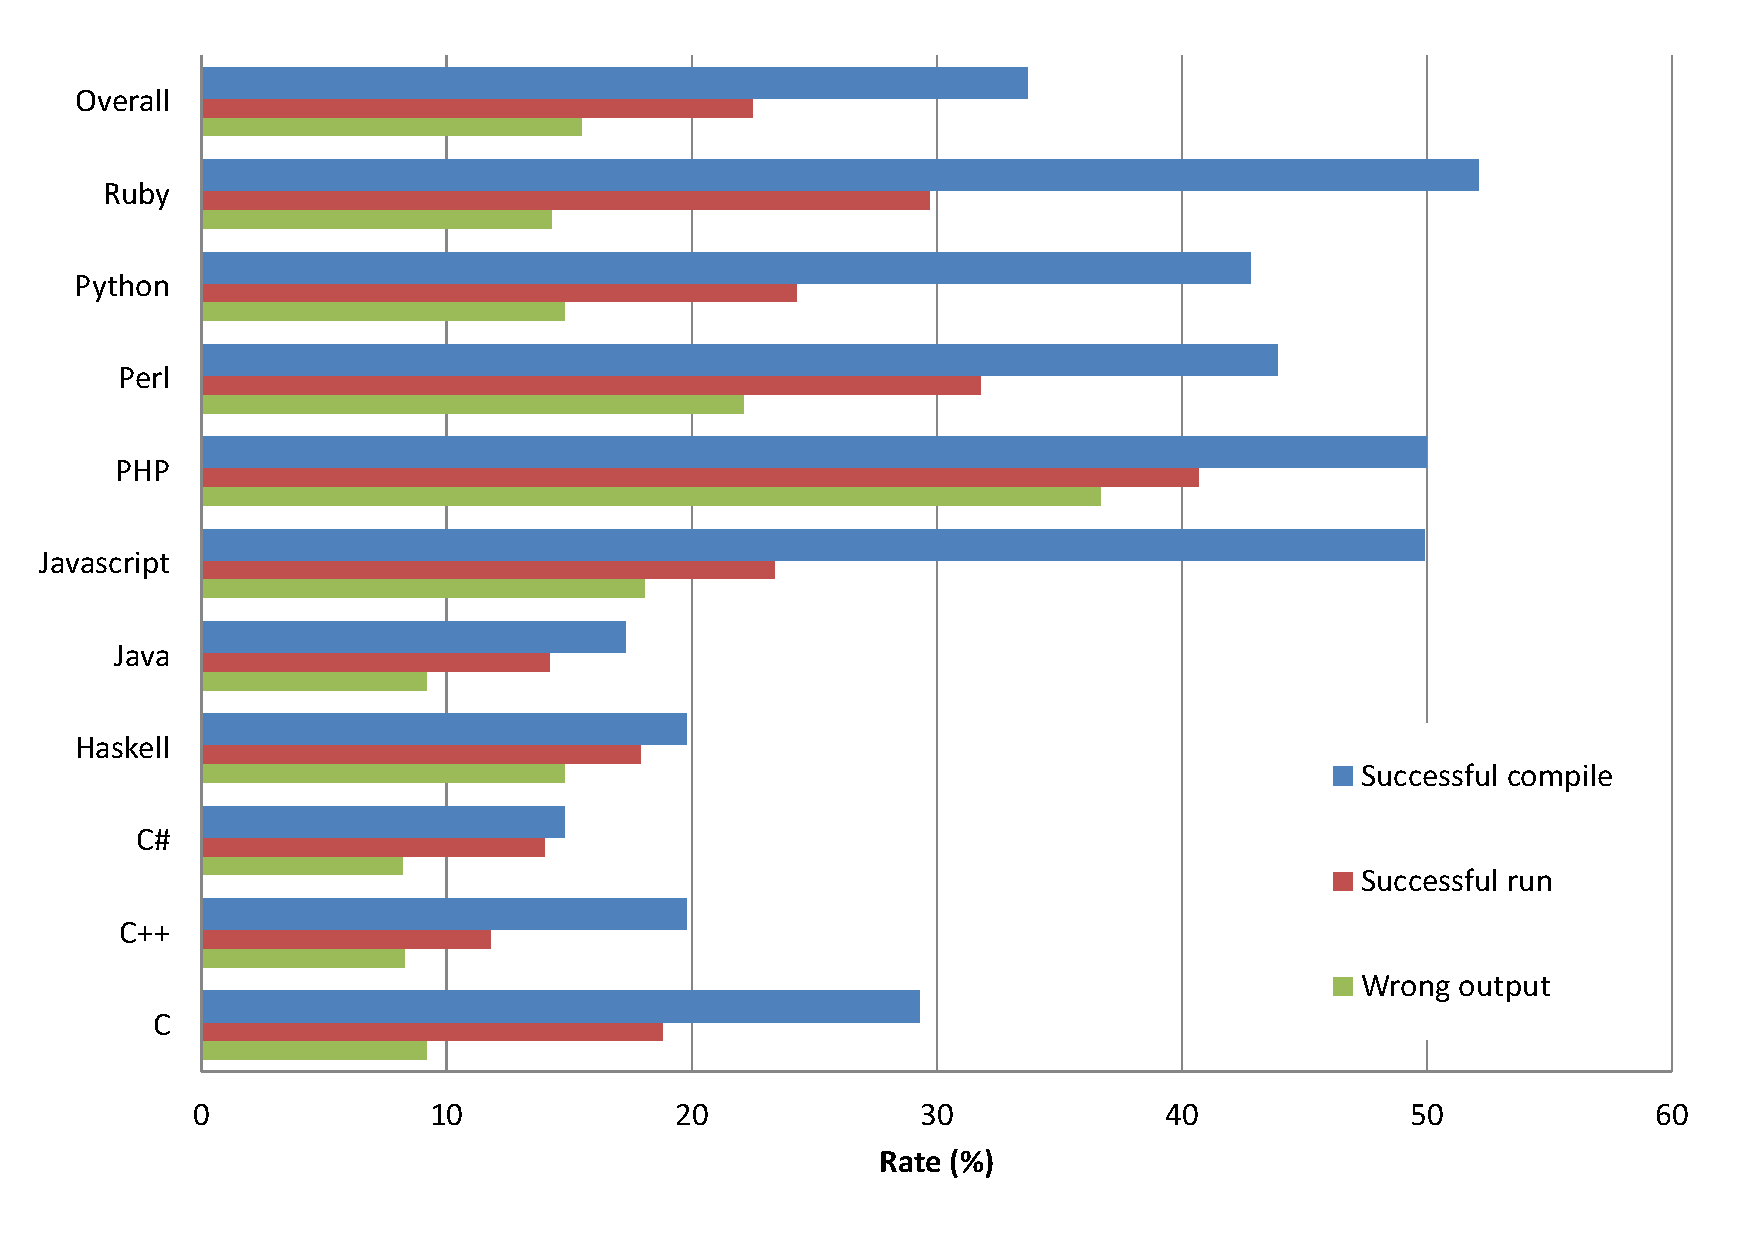
\includegraphics[width=0.95\textwidth]{chart}
        \end{center}
        \caption{Failure modes for each phase per language and overall.}
        \label{fig:results}
\end{figure*}

The aggregate results per language are summarized in Figure~\ref{fig:results}
in the form of {\em failure modes}:
successful compiles or executions, which consequently failed to catch an
erroneous program and resulted in wrong results.
The rationale behind this depiction is that the later in the software
development life cycle an error is caught the more damaging it is.
The denominator used for calculating the percentages also includes
fuzzing operations that resulted in correct results.
Therefore, the numbers also reflect the programming language's
information density:
in our case the chance that a fuzz will not affect the program's operation.

The figure confirms a number of intuitive notions.
Languages with strong static typing (Java, Haskell, C++)
caught more errors at compile time than languages
with weak or dynamic type systems
(Ruby, Python, Perl, {\sc php}, and JavaScript).
Somewhat predictably, C fell somewhere in the middle,
confirming a belief that its type system is not as strong
as many of its adherents (including this article's first author)
think it is.
However, C produced a higher number of run-time errors,
which in the end resulted in a rate of incorrect output
similar to that of the other strongly-typed languages.

A picture similar to that of compile-time errors
is also apparent for run time behavior.
Again, code written in weakly-typed languages are more probable to run without
a problem than code written in languages with a strong type system.
As one would expect these two differences result in a higher rate of
wrong output from programs written in languages with weak typing.
With an error rate of 37\% for {\sc php} against one of 8\% for
C++ and C\#, one would be foolish indeed to write a defibrillator's
software in {\sc php}.

Overall, the figures for dynamic scripting languages show a far larger
degree of variation compared to the figures of the strongly static typed
ones.
This is probably a result of a higher level of experimentation
associated with scripting language features.

\begin{table*}
\begin{center}
\begin{tabular}{ l r r r|r r r|r r r|r r r|r r r}
& \multicolumn{3}{c}{IntPert (\%)} & \multicolumn{3}{c}{IdSub (\%)} & \multicolumn{3}{c}{SimSub (\%)} & \multicolumn{3}{c}{RandCharSub (\%)} & \multicolumn{3}{c}{RandTokenSub (\%)}\\ 
	       & com  & run  & out  & com  & run  & out  & com  & run  & out  & com & run   & out  & com  & run  & out\\
\hline													
C & 100.0 & 52.6 & 34.0 & 16.6 & 14.0 & 3.6  & 20.6 & 16.6 & 7.0  & 7.3 & 7.3 & 1.1  & 5.4 & 5.1 & 1.7 \\
C++ & 91.7 & 47.2 & 41.0  & 5.6 & 4.9 & 1.0  & 8.3 & 7.1 & 4.0  & 3.7 & 3.7 & 0.3  & 2.6 & 2.4 & 1.1 \\
C\# & 69.8 & 65.2 & 53.2  & 6.9 & 6.9 & 0.3  & 7.7 & 7.4 & 1.4  & 4.0 & 4.0 & 0.1  & 3.0 & 3.0 & 0.3 \\
Haskell & 89.4 & 84.0 & 73.7  & 4.0 & 1.9 & 1.5  & 13.4 & 11.2 & 9.1  & 3.7 & 3.4 & 1.1  & 3.5 & 3.2 & 1.5 \\
Java & 100.0 & 82.5 & 62.1  & 5.1 & 3.6 & 0.7  & 7.9 & 6.4 & 3.3  & 3.1 & 3.0 & 0.1  & 2.3 & 1.9 & 0.1 \\
Javascript & 100.0 & 79.7 & 73.7  & 65.9 & 18.4 & 12.7  & 57.2 & 22.9 & 17.8  & 30.9 & 9.6 & 1.7  & 15.0 & 5.7 & 3.9 \\
{\sc php} & 99.2 & 87.5 & 71.3  & 56.4 & 34.1 & 31.0  & 46.2 & 39.7 & 38.3  & 37.4 & 32.7 & 30.9  & 25.7 & 23.7 & 22.6 \\
Perl & 100.0 & 91.0 & 68.9  & 57.9 & 29.3 & 21.9  & 44.3 & 27.3 & 16.8  & 15.1 & 11.6 & 4.9  & 18.2 & 14.2 & 9.2 \\
Python & 100.0 & 75.3 & 60.9  & 43.3 & 17.3 & 4.7  & 45.2 & 23.6 & 13.6  & 18.3 & 6.9 & 0.7  & 20.7 & 10.6 & 4.9 \\
Ruby & 100.0 & 91.1 & 59.5  & 52.3 & 11.8 & 2.7  & 58.0 & 27.0 & 10.9  & 27.6 & 14.7 & 2.4  & 33.4 & 15.8 & 4.8 \\
\textbf{Mean} & \textbf{95.1} & \textbf{74.5} & \textbf{58.7}  & \textbf{30.6} & \textbf{14.0} & \textbf{7.8}  & \textbf{30.3} & \textbf{18.7} & \textbf{12.1}  & \textbf{15.1} & \textbf{9.7} & \textbf{4.3}  & \textbf{12.8} & \textbf{8.5} & \textbf{5.0} \\
\end{tabular}
\end{center}
\caption{Failure modes for each language, fuzz operation, and phase (successful compilations, runs, and wrong output).}
\label{tbl:aggregated-per-language}
\end{table*}

The results for each fuzz type, phase, and language are summarized in
Table~\ref{tbl:aggregated-per-language}.
Predictably, the off-by-one integer perturbation ({\em IntPert})
was the fuzz that
compilers found most difficult to catch and the one that resulted
in most cases of erroneous output.
The C\# compiler seems to behave better than the others in this area,
having a significantly lower number of successful compilations than the
rest.
However, this did not result in a similarly good performance rank
regarding lack of erroneous output.

Identifier substitution ({\em IdSub}) and similar token substitution
({\em SimSub}) resulted in almost equal numbers of compilation failures.
Although one might expect that {\em IdSub} would be more difficult
to detect than the wider-ranging {\em SimSub},
our fuzzer's treatment of reserved words as identifiers
probably gave the game away.
Nevertheless, {\em SimSub} resulted in a significantly higher number
of successful runs and erroneous results.
The erroneous results for {\em SimSub} were dramatically higher
than those for {\em IdSub} in the case of
languages with a more imaginative syntax, like Python, Haskell, and Ruby.

The random character substitution fuzz was the one that resulted
in the lowest number of erroneous results.
However, it wrecked havoc with {\sc php}s compilation and output,
and JavaScript's compilation.
This could be associated with how these languages treat source code
with non-{\sc ascii} characters.

Finally, the random token substitution resulted in the lowest number
of successful compilations or runs and consequently
also a low number of erroneous results.
{\sc php} performed particularly badly in this area indicating a
dangerously loose syntax.

\section{Related Work} % {{{1
\label{sec:related}
Comparative language evaluation has a long and colorful history;
see for instance reference \cite{Ker81} and the reference therein.

Fuzzing as a technique to investigate the reliability of software
was first proposed in an article by Miller and his colleagues~\cite{MFS90}.

In this paper they tested the common collection of {\sc unix}
utilities in various operating systems and architectures and discrovered that
25-33\% of these, are crashing under certain conditions. To perform these tests
they implemented automation shell scripts and a fuzzer, a program that generated
random character sequences according to certain specifications.

Fuzzing is used mainly to detect software security vulnerabilities and 
improve overall reliability \cite{TJC08,GODE07}. Several tools and techniques \cite{WWGZ11}
have been developed, introducing concept like \textit{directed fuzz testing} \cite{GLRI09}.

Our approach fuzzes the program with pseudo-random
perturbations based in same cases on knowledge of
lexical tokens. This can result in a large number of failures.

An alternative approach, {\em grammar-based white box fuzzing} \cite{God08},
takes into account the input language's grammar to fuzz the input in
ways that are syntactically correct.
This results in a higher rate of successful fuzzing and the location
of deeper problems.

Another interesting approach is H-fuzzing \cite{ZWZH11}, which is a heuristic method that examines the execution paths
of the program to achieve higher path coverage. All these approaches are based on the fact that it is practically impossible to detect all
execution paths and all program inputs to fully test the validity and the reliability of a program.

Random Testing \cite{HAM06} seems to be promising solution that can partially deal with this problem,
but still it is not widely adopted outside the academic fields \cite{GGBO07}, since the techniques it 
introduces are difficult to be applied in complex systems and achieve good code coverage, if so at a significant cost \cite{RAWO06}.

The above case is made worse with the use of complex refactorings \cite{Fow00} in day-to-day programming. Refactorings are beneficial, but they are programs integrated in {\sc ide}s and also have bugs \cite{DDGM07}. Every bug results in corrupted code, which is very difficult to detect, especially for the case of dynamic langugages \cite{SCHA12,FFM11}.

Our experiment aims to exhibit the fault tolerance \cite{LYU95,KOKR07} of each language and use their features such as 
their type systems to our advantage. 

Type systems are usually realized as type checkers in compilers and linkers of programming languages. They are categorized as static and dynamic. \textit{Static typing} implies static type checking. In other words, the ability of a programming language's compiler to know all the data types that are used in a program, and guarantee that they are correct at compile time. \textit{Dynamic typing} is exactly the opposite. The languages that are dynamically checked perform run-time checks in order to ensure consistent type use. 

In addition, a programming language is called safe, when it protects its own abstractions. For example, a programming language that provides an abstraction for arrays, is considered safe, if it performs boundary checking upon access. Consequently, Java is a statically checked and safe programming language, while C/C++ are statically checked and unsafe. On the other hand, Perl and Lisp are dynamically checked and safe \cite{Pie02}.

Statically typed languages are in general resilient to several fuzzing techniques, since the compiler catches all syntax or type errors and fail the compilation process. Dynamic languages like python, perl and ruby are evaluating many things at runtime and usually they fail upon execution or produce corrupted output.

Different behaviour and productivity issues of the programmers are also pointed out in reference \cite{RWSB68}, which states that high-level abstractions of PL/I. helped programmers to write fewer program statements, but with higher frequency of errors. To support this, a programmer implemented twice seven benchmark problems in PL/I and in one other language; Cobol, Fortran and Jovial. The aforementioned publication is very interesting, because it correlates directly the language abstractions with the user productivity and efficiency, in terms of valid program code, with the comparison of programming languages. It is an experinment similar to the one presented in this research.

\section{Conclusions and Further Work} % {{{1
\label{sec:conclusions}

The work we described in this study cries to be extended
by applying it on a larger and more diverse corpus of programming tasks.
It would also be interesting to test a wider variety of languages.
Although Haskell performed broadly similar to the other strongly-typed
languages in our set we would hope that other declarative languages
would exhibit more interesting characteristics.
The fuzz operations can be also extended and be made more realistic,
perhaps by implementing a mixture based on data from actual programming
errors.

In this study we tallied the failure modes associated with each
languages and fuzz operation and reported the aggregate results.
Manually analyzing and categorizing the failure modes associated
with each language and fuzz operation is likely to produce
interesting insights, as well as feedback that can drive the
construction of better fuzz operations.

We already mentioned in Section~\ref{sec:results} that the
large degree of variation we witnessed among the scripting
language results may be a result of those languages
more experimental nature.
More interestingly, this variation also suggests that
comparative language fuzz testing of the type we performed
can also be used to objectively evaluate programming language
designs.

Probably the most significant outcome of our study is the
fact that comparative language fuzz testing is a
legitimate technique for evaluating programming language designs.
This opens the door into two broad research directions.

The first research direction involves the comparative evaluation
of programming languages using objective criteria,
such as the response to fuzzing of code implementing the same functionality
in diverse languages.
This is made significantly easier through the publication of
tasks implemented in numerous programming languages on the
{\em Rosetta Code} site.
Our community should therefore expend effort to contribute to
the site's wiki, increasing the trustworthiness and diversity of
the provided examples.

The second research strand involves the systematic study of
language design by using methods from the fields of reliability engineering
and software testing.
Again, fuzzing is just one technique, others could be inspired from
established methods like
hazard analysis,
fault tree analysis, and
test coverage analysis.

\acks

We would like to thank Florents Tselai for significant
help in the porting and implementation of the
{\em Rosetta Code} tasks in our environment,
and the numerous contributors of {\em Rosetta Code} for
making their efforts available to the public.

This work is supported by European and Greek national funds
under the ``Thalis'' action, {\sc stereo} research program
(2012SE24580099).

\paragraph{Code Availability} The source code for
the implemented tasks,
the fuzzer,
the language-specific methods, and
the driver are maintained on GitHub, and
will be made publicly available as open source software
before the paper is published.
% XXX STEREO

% We recommend abbrvnat bibliography style.

\bibliographystyle{abbrvnat}
\bibliography{fuzzer}

% The bibliography should be embedded for final submission.

%\begin{thebibliography}{}
%\softraggedright

%\bibitem[Smith et~al.(2009)Smith, Jones]{smith02}
%P. Q. Smith, and X. Y. Jones. ...reference text...

%\end{thebibliography}

\end{document}
